\section{The CAMS Framework}
The CARP Mobile Sensing (CAMS) Framework\footnote{\url{https://github.com/cph-cachet/carp.sensing-flutter/wiki}} is a Flutter framework for adding digital phenotyping capabilities to a mobile-health app. An integration for the \textit{Mobility Features Package} into the CAMS Framework is a future goal beyond this thesis, but describing CAMS will provide some insight into the direction of the package. 

\subsection{The Goal of CAMS}
CAMS is designed to collect research-quality sensor data from the many smartphone data channels such as sensors and location data, in addition to external sensors that the phone is connected to, such as wearable devices. The main focus of the framework is to allow application programmers to design and implement a custom mobile health app without having to start from scratch, with regards to the sensor integration, by enabling the programmers to add an array of mobile sensing capabilities in a flexible and simple manner. This would include adding support for collecting health-related data channels such as \textit{ECG}, \textit{GPS}, \textit{Sleep}, \textit{Activity}, \textit{Step Count} and much more. Additionally, to format the resulting data according to standardized health data formats (like \textit{Open mHealth} schemas \footnote{\url{https://www.openmhealth.org/documentation/#/schema-docs/schema-library}}. Last but not least, the collected data should be uploaded to a server, using an API (such as \textit{REST}), and should come in a standardized format such that it may easily be imported for data analysis. To include as many data channels as possible the application should also be able to support different wearable devices for ECG monitoring and activity tracking. Hence, the focus is on software engineering support in terms of a solid programming API and a runtime execution environment, that is being maintained as the underlying mobile phone operating systems and APIs are evolving. Moreover, the focus is on providing an extensible API and runtime environment, which together allow for adding application-specific data sampling, wearable devices, data formatting, data management, and data uploading functionality to an application. In addition, in order to reduce the number of integrations needed, the framework must be cross-platform such that it supports both Android and iOS, without having a codebase for each platform.

\subsection{The CAMS Domain Model}
The data collection pipeline is defined by a \textit{Study} which contains all the information needed to conduct a real-world study, which includes the collection of certain data types with a set of rules and saving it somewhere. 

\begin{figure}[h]
    \centering
    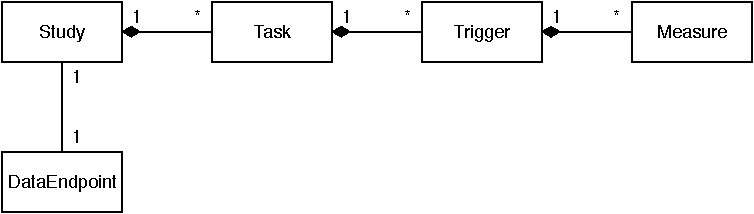
\includegraphics[width=0.8\textwidth]{images/CAMS-UML.pdf}
    \caption{A UML diagram of the \textit{CAMS} Domain Model.}
    \label{fig:cams_uml}
\end{figure}

Concretely, a \textit{Study} holds a set of \textit{Triggers}, which define \textit{when} sampling is carried out, such as by scheduling sampling at  given time each day, or when a certain event is registered, such as entering a specific \textit{GeoFence}\footnote{\url{https://developers.google.com/location-context/geofencing}}. 

Each \textit{Trigger} holds one or more \textit{Tasks}, each of which define which \textit{Measures} should run simultaneously. In addition, a \textit{Task} also defines whether or not data is sampled in the background, or whether the user needs to interact with the device in order to perform sampling. 

Each \textit{Task} holds a set of \textit{Measures} each of which defines what to sample, i.e. which data channel to listen to. Lastly, a \textit{Study} also holds a reference to the \textit{DataEndpoint} specifying which where data ends up, i.e. by uploading it to a server.

